\documentclass[10pt]{beamer}

\usetheme[progressbar=frametitle]{metropolis}
\usepackage{appendixnumberbeamer}

\usepackage{booktabs}

\usepackage{pgfplots}
\usepackage{minted}
\usepgfplotslibrary{dateplot}
\usepackage{dirtree}

\usepackage[style=authoryear,backend=biber, bibstyle=authoryear]{biblatex}
\addbibresource{progtech.bib}% Syntax for version >= 1.2

\usepackage{xspace}
\newcommand{\themename}{\textbf{\textsc{metropolis}}\xspace}

\title{Implementing a \textcite{holt_risk_2002} Multiple Price List lottery in oTree}
% \date{\today}
\date{}
\author{Olaf Ghanizadeh}
% \titlegraphic{\hfill\includegraphics[height=1.5cm]{logo.pdf}}
\setbeamercolor{background canvas}{bg=white}


\setminted[python]{
  frame=lines,
  framesep=2mm,
  baselinestretch=1.2,
  fontsize=\footnotesize,
  linenos
}

\usepackage{graphicx}
\usepackage{float}

\begin{document}

\maketitle

\section{What is oTree?}

\begin{frame}[fragile]{What is oTree?}

  \begin{itemize}
    \item Open Source framework to create behavioral economics experiments, \textcite{chen_otreeopen-source_2016}
    \item Python based, uses Django to create a web application
    \item Bootstrap 4 for styling
    \item Encourages object-oriented programming, extensive use of classes and methods in order to avoid code duplication
  \end{itemize}

\end{frame}

\begin{frame}{Basic Strucutre}
  \dirtree{%
  .1 oTree.
  .2 settings.py.
  .2 hl\_mpl.
  .3 templates.
  .4 hl\_mpl.
  .5 template files.
  .3 config.py.
  .3 models.py.
  .3 pages.py.
  .3 utils.py.
  }
\end{frame}

\section{How does oTree work?}
\begin{frame}[fragile]{\mintinline{python}{models.py}}
  \begin{minted}{python}
    class Subsession(BaseSubsession):
    """Create the session to be played"""
      n = self.session.config['num_choices']
      # Store in session variables
      self.session.vars['probs'] = probs
      def creating_session(self):
      """Session variables that holds for all players in this session"""
        for p in self.get_players():
        """Each player, p, in the session, self"""
    
    class Group(BaseGroup):
      """If we wanted to have players in different  groups"""
        pass
  \end{minted}
\end{frame}

\begin{frame}[fragile]{\mintinline{python}{models.py}}
  In \mintinline{python}{models.py} we execute most of our code:
  \begin{minted}{python}
    class Player(BasePlayer):
    """We execute what goes for each player."""
      name = models.StringField()
  \end{minted}

We register the fields that will be exposed on the front-end, and the variables that will be stored in each 'player object'

\begin{minted}{python}
    def set_payoffs(self):
\end{minted}
A method within the Player Class where we can set the payoff for each player. We need to call this method for payoffs to be set. In my project it is called before the user sees the final results page. 
\end{frame}

\begin{frame}[fragile]{\mintinline{python}{pages.py}}
  In \mintinline{python}{pages.py} we create the pages that will be shown to the user, define the forms, expose variables for the front end and so on. Each instance of \mintinline{python}{Page} gets linked to a HTML file in the templates folder. 
  \begin{minted}{python}
# Class for the IntroPage. Inherits attributes from Page Class
class IntroPage(Page):
    # Get forms to be displayed on IntroPage
    form_model = 'player'
    form_fields = ['name', 'risk']
  \end{minted}

We register the fields that will be exposed on the front-end, and the variables that will be stored in each 'player object'
\end{frame}

\begin{frame}[fragile]{\mintinline{python}{pages.py}}
  \begin{minted}{python}
# Class for the DecisionPage. Inherits attributes from Page Class
class DecisionPage(Page):
    form_model = 'player'

    ...

    # Triggers the function that set draws the payoff of the
    #user before the user is taken to the result page. This
    # should be changed if we were to make a game with several rounds.
    def before_next_page(self):
        self.player.set_payoffs()
  \end{minted}

We call the \mintinline{python}{self.player.set_payoffs()} before the next page is loaded to set the payoffs for the individual player. 
\end{frame}



\begin{frame}[fragile]{Templates}
  \begin{itemize}
    \item HTML Templates made dynamic with Django Template Language (DTL): \mintinline{python}{{{player.name}}}
    \item Extendable with JavaScript
  \end{itemize}
\end{frame}


\section{Experiment}

\begin{frame}{Experiment}

  \begin{itemize}
    \item A simplified version of the experiment popularized in \textcite{holt_risk_2002}.
    \item An approach to elicit individual preferences for risk in various contexts.
    \item Assumes that Constant Relative Risk Aversion holds
  \end{itemize}
  
\end{frame}

\begin{frame}{Goal in our experiment}
  \begin{quote}
    Does the participant choose differently from their indicated risk preferences? 
  \end{quote}
\end{frame}

\begin{frame}
  \begin{itemize}
    \item A risk-neutral user should consider the expected values of the different outcomes, and maximize it for each choice. 
    \item In our experiment that is the sequence: AAA/BBBBB
    \item The number of safe choices (A), or the switching point, can be used to estimate risk preferences and the parameters of an individual utility function. 
  \end{itemize}
\end{frame}

\begin{frame}
    \small
    \begin{table}[H]
  \centering
  \caption{Probabilities, choices and expected values}
    \begin{tabular}{ccccccccc}
      \toprule
         $p$ &  $1-p$ & $A_{High}$ & $A_{Low}$ & $B_{High}$ & $B_{Low}$ & $E[A]$ &   $E[B]$ & Difference \\
      \midrule
       0.125 &  0.875 &        200 &       160 &        385 &        10 &  165.0 &   56.875 &    108.125 \\
       0.250 &  0.750 &        200 &       160 &        385 &        10 &  170.0 &  103.750 &     66.250 \\
       0.375 &  0.625 &        200 &       160 &        385 &        10 &  175.0 &  150.625 &     24.375 \\
       0.500 &  0.500 &        200 &       160 &        385 &        10 &  180.0 &  197.500 &    -17.500 \\
       0.625 &  0.375 &        200 &       160 &        385 &        10 &  185.0 &  244.375 &    -59.375 \\
       0.750 &  0.250 &        200 &       160 &        385 &        10 &  190.0 &  291.250 &   -101.250 \\
       0.875 &  0.125 &        200 &       160 &        385 &        10 &  195.0 &  338.125 &   -143.125 \\
       1.000 &  0.000 &        200 &       160 &        385 &        10 &  200.0 &  385.000 &   -185.000 \\
      \bottomrule
    \end{tabular}
\end{table}
\end{frame}





\section{Acknowledgements}
\begin{frame}[fragile]{Acknowledgements}
  \begin{itemize}
    \item Simplified version of experiment
    \item Should record if the user decides to change their mind. I.e. choosing $A \rightarrow B \rightarrow A$ in a specific choice. 
    \item Code error with $> 9$ choices.
    \item Should include several rounds and treatments
    \item Incentives are not compatible: Limited value of resulting data
  \end{itemize}
\end{frame}

\section{Data Analysis}

\begin{frame}{Choices of 20 participants}
  \begin{figure}[H]
  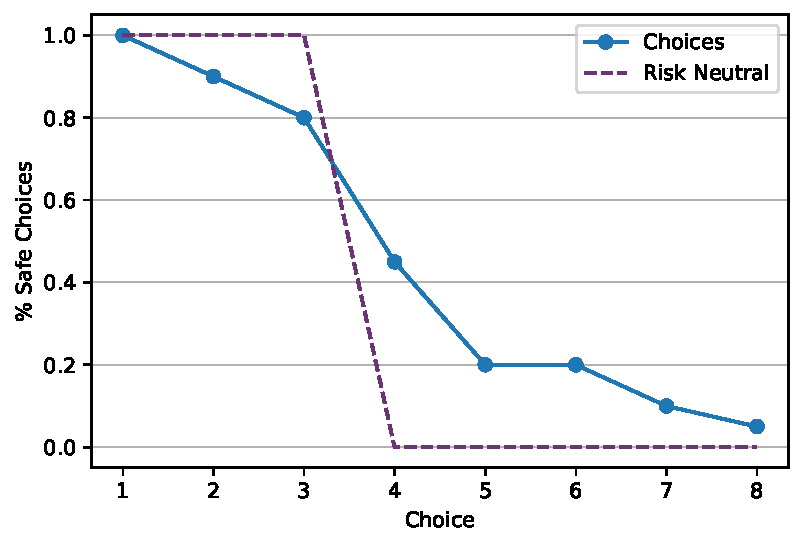
\includegraphics[width=0.9\columnwidth]{graphics/aggregate_plot.pdf}
  \caption{Choices made compared to a 'risk neutral' profile}
\end{figure}
\end{frame}

\begin{frame}{Flask Application}
  \url{https://progtech-flask-app.herokuapp.com/}
  \begin{itemize}
    \item Passes the data from Pandas to Flask
    \item Using d3.js for visualization
  \end{itemize}
\end{frame}


\begin{frame}{A random sample}
  \resizebox{\textwidth}{!}{
    \begin{tabular}{lllllllll}
\toprule
   Indicated & Choice 1 & Choice 2 & Choice 3 & Choice 4 & Choice 5 & Choice 6 & Choice 7 & Choice 8 \\
\midrule
 Risk Averse &        A &        A &        A &        A &        A &        A &        B &        B \\
\bottomrule
\end{tabular}

  }
\end{frame}

\begin{frame}{Random sample visualized}
  \begin{figure}[H]
  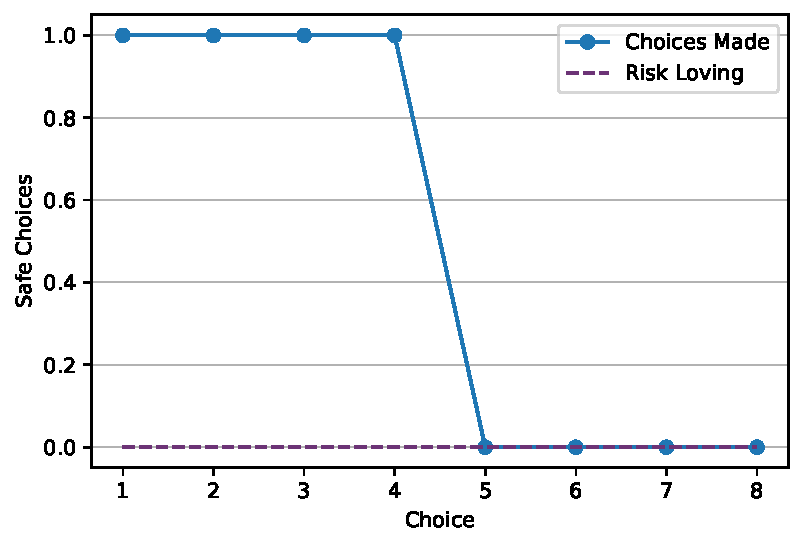
\includegraphics[width=0.9\columnwidth]{graphics/random_plot.pdf}
  \caption{Choices made compared to the indicated profile}
\end{figure}
\end{frame}

\begin{frame}
  \Huge\input{includes/drawn_name.txt}
\end{frame}












\begin{frame}{References}
  \printbibliography[heading=none]
\end{frame}




{\setbeamercolor{palette primary}{fg=black, bg=yellow}
\begin{frame}[standout]
  Questions?
  \begin{description}
      \item[Experiment code:] \url{https://github.com/olafghanizadeh/hl_mpl}
      \item[Project files:] \url{https://github.com/olafghanizadeh/hl_mpl}
  \end{description}
\end{frame}
}





\end{document}
